\begin{figure}[!h]
    \centering
    \resizebox{0.87\textwidth}{!}{
        \begin{tikzpicture}[mindmap,
        level 1 concept/.append style={level distance=130,sibling angle=120},
        level 2/.append style={level distance=100,sibling angle=120},
        ]
        \path[mindmap,concept color=black,text=white]
        node[concept] {Function}
        [clockwise from=0]
        child[concept color=blue,sibling angle=0,text=black]{
          node[concept] (periodic) {Periodic\\Functions}
          [clockwise from=0]
          child[concept color=green!50!black,sibling angle=90] {
              node[concept] (trigFunctions) {Trig.\\Functions}
              [clockwise from=55]
              child[concept color=green!50!black,sibling angle=90] {
                node[concept] (tangent) {Tangent}
              }
              child[concept color=green!50!black,sibling angle=90] {
                node[concept] (sine) {Sine}
              }
              child[concept color=green!50!black,sibling angle=90] {
                node[concept] (cosine) {Cosine}
              }
          }
          child[concept color=blue,sibling angle=98,level distance=110,font=\fontsize{8pt}{10pt}\selectfont] {
            node[concept,scale=1.4] (oscillations) {Oscillations}
            [clockwise from=-90]
            child[concept color=blue,sibling angle=45,level distance=80,font=\fontsize{4pt}{6pt}\selectfont] {
              node[concept,scale=1.5] (frequency) {Frequency}
            }
            child[concept color=blue,sibling angle=45,level distance=80,font=\fontsize{4pt}{6pt}\selectfont] {
              node[concept,scale=1.5] (amplitude) {Amplitude}
            }
          }
        };

        \begin{pgfonlayer}{background}
%        \draw [color=blue,ultra thick,looseness=1.5,<-] (arcLength) [out=-22, in=-45] to (radians);
        \draw [left color=blue, right color=green!50!black, draw=white,
               decorate,decoration=circle connection bar]
               (oscillations.east) -- (sine.south);
        \draw [left color=blue, right color=green!50!black, draw=white,
               decorate,decoration=circle connection bar]
               (oscillations.east) -- (cosine.south);
%        \draw [color=blue,ultra thick,looseness=1.5,<-] (arcArea) [out=0, in=-45] to (radians);
        \end{pgfonlayer}


        \end{tikzpicture}
    }
\end{figure}

%=========================================================================
% Start of
%=========================================================================
\preClass{Basic Trigonometry}

\begin{problem}
\item A circle of radius $r$ is centered at the origin, and a ray
  originates from the origin at a given angle, $\theta$. The ray
  passes through the circle at the coordinate $(x,y)$. A function of
  $\theta$ can be defined in terms of the coordinate.

  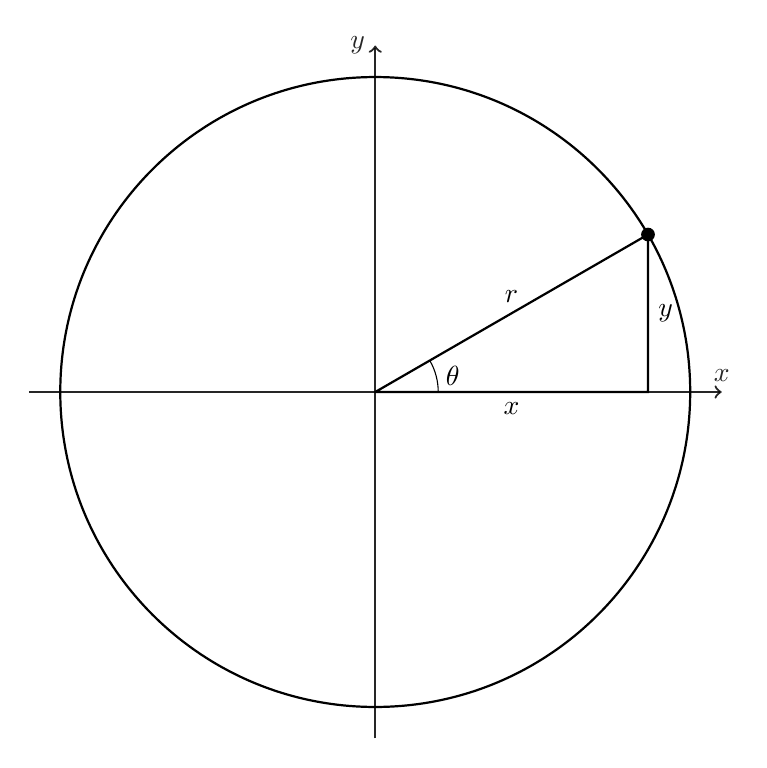
\begin{tikzpicture}[y=4cm, x=4cm,font=\sffamily]
      \draw[thick,opacity=0.85,->] (0, -1.1) -- (0,1.1) node[anchor=east] {$y$};
      \draw[thick,opacity=0.85,->] (-1.1, 0) -- (1.1,0) node[anchor=south] {$x$};
      \draw[thick] (1,0) arc (0:360:1);
      \draw[thick] (0,0) -- (30:1) node[midway,anchor=south] {$r$}
          -- ++(-90:0.5) node[midway,anchor=west] {$y$}
          -- (0,0) node[midway,anchor=north] {$x$};
      \draw[fill=black] (30:1) circle (0.02);
      \draw[text=black] (0:0.2) arc (0:30:0.2) node[midway,anchor=west] {$\theta$};
    \end{tikzpicture}


  \begin{subproblem}
  \item A function, sine, is defined to be
    \begin{eqnarray*}
      \sin(\theta) & = & \frac{y}{r}.
    \end{eqnarray*}
    Determine the formula for the value of $y$ given $r$ and $\theta$
    in terms of the sine function.
    \sideNote{Solve the equation above for $y$.}
    \vfill
  \item A function, cosine, is defined to be
    \begin{eqnarray*}
      \cos(\theta) & = & \frac{x}{r}.
    \end{eqnarray*}
    Determine the formula for the value of $x$ given $r$ and $\theta$
    in terms of the cosine function.
    \sideNote{Solve the equation above for $x$.}
    \vfill
  \end{subproblem}

\end{problem}


\actTitle{Basic Trigonomety}
\begin{problem}
\item Answer each of the following questions where the given point is $P(2,4)$.
  \begin{subproblem}
  \item Make a sketch of the coordinate plane and include the point
    $P(2,4)$. Draw the ray from the origin to the point.
    \sideNote{Label your axes and annotate your plot.}
    \vfill
  \item Add a circle to your sketch whose center is the origin and goes
    through the point. Label the angle $\theta$ as the angle between
    the ray and the $x$-axis.
  \item What is the radius of the circle? (Add a label to your plot for the radius.)
    \vspace{2em}
  \item Determine the values of the sine and cosine for the angle.
    \begin{eqnarray*}
      \sin(\theta) & = & \\ [10pt]
      \cos(\theta) & = &
    \end{eqnarray*}
  \end{subproblem}

\clearpage

\item Different points are given below. For each point assume it is
  on the edge of a circle whose center is at the origin.
  Determine the radius of the circle as well as the value of the
  sine and cosine of the angle associated with each point on its circle.
  \begin{subproblem}
  \item $P(1,0)$
    \vfill
  \item $P(0,1)$
    \vfill
  \item $P(-1,0)$
    \vfill
  \item $P(0,-1)$
    \vfill
  \item $P\left(\frac{\sqrt{2}}{2},\frac{\sqrt{2}}{2}\right)$
    \vfill
  \end{subproblem}

\clearpage

\item In each item below some information is given about an angle.
  Use the information to determine the sine, cosine, and tangent of the
  angle.
  \begin{subproblem}
    \item The angle is in the first quadrant and $\cos(\theta)=0.3$.
      \vfill
    \item The angle is in the third quadrant and $\sin(\theta)=-0.25$.
      \vfill
    \item The angle is in the fourth quadrant and $\sin(\theta)=-0.4$.
      \vfill
    \item The angle is in the second quadrant and $\cos(\theta)=-0.8$.
      \vfill
  \end{subproblem}

\end{problem}

\postClass

\begin{problem}
\item Briefly state two ideas from today's class.
  \begin{itemize}
  \item
  \item
  \end{itemize}
  \item The circle below is centered at the origin and has a radius of
    one.

    %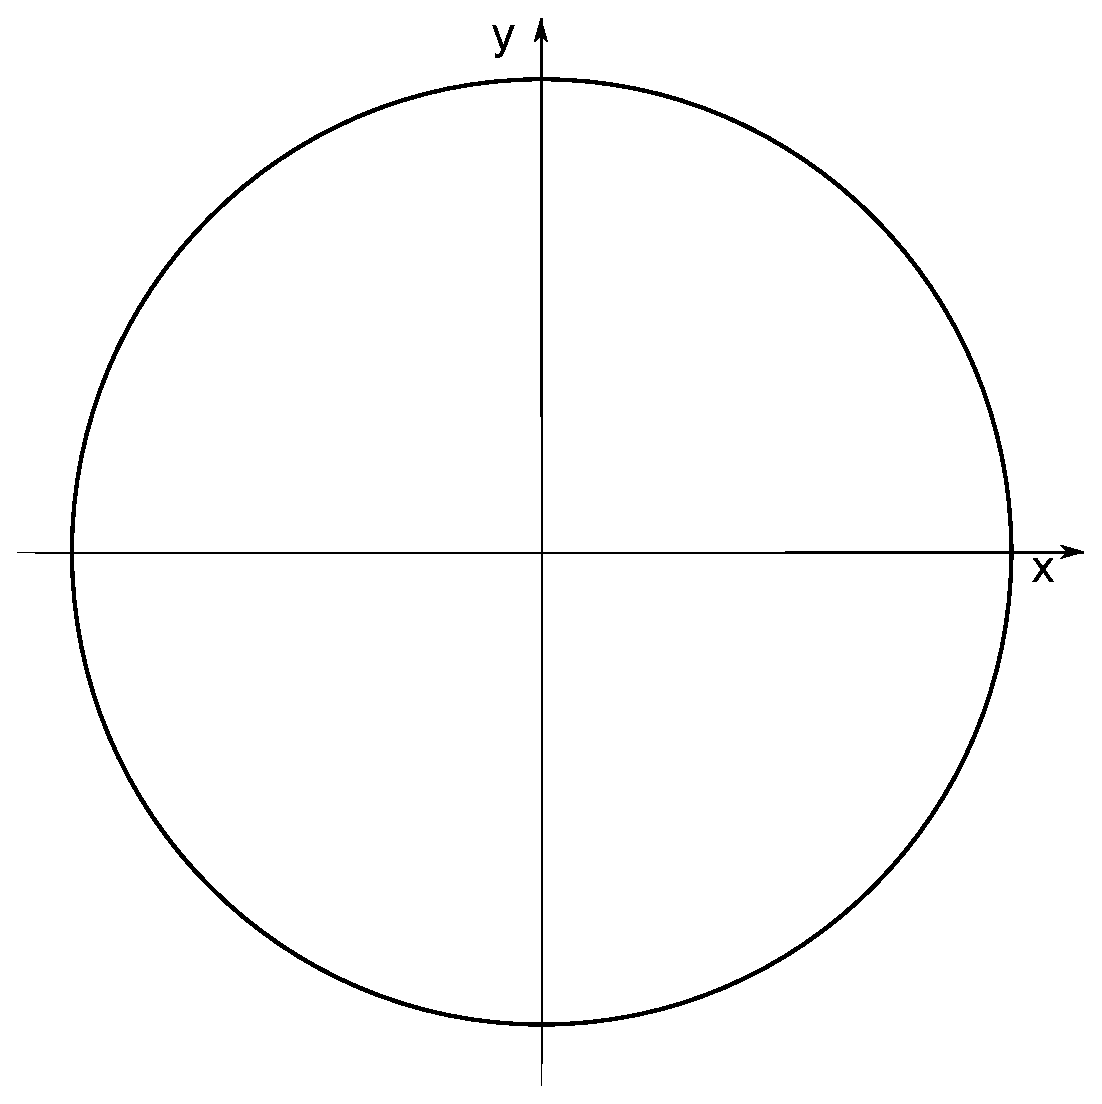
\includegraphics[width=16cm]{trig/img/blankCircle}
    \begin{tikzpicture}[y=6cm, x=6cm,font=\sffamily]
        \draw[thick,opacity=0.85,->] (0, -1.1) -- (0,1.1) node[anchor=east] {$y$};
        \draw[thick,opacity=0.85,->] (-1.1, 0) -- (1.1,0) node[anchor=south] {$x$};
        \draw[thick] (1,0) arc (0:360:1);
      \end{tikzpicture}

    \begin{subproblem}
    \item Mark the locations on the circle whose associated angles are
      0, $\pi/4$, $\pi/2$, $3\pi/4$, $\pi$, $5\pi/4$, $3\pi/2$, and
      $7\pi/4$.
      Determine the coordinates for the points.
      (Label the points and annotate your plot.)
    \item Determine the $(x,y)$ coordinates for each angle.
    \item Determine the cosine and sine of each angle.
    \end{subproblem}
\end{problem}


%%% Local Variables:
%%% mode: latex
%%% TeX-master: "../labManual"
%%% End:


%=========================================================================
% Start of 
%=========================================================================
\preClass{Title}

\begin{problem}
\item
\end{problem}


\actTitle{title}
\begin{problem}
\item 
  \begin{subproblem}
    \item
  \end{subproblem}
\end{problem}

\postClass

\begin{problem}
\item Briefly state two ideas from today's class.
  \begin{itemize}
  \item 
  \item 
  \end{itemize}
\item 
  \begin{subproblem}
    \item
  \end{subproblem}
\end{problem}


%%% Local Variables:
%%% mode: latex
%%% TeX-master: "../labManual"
%%% End:



%=========================================================================
% Start of activity on reference angles
%=========================================================================
\preClass{Reference Angles}

\begin{problem}
\item Determine the sine and cosine of the angle $\frac{\pi}{4}$.
  \vfill
\item Determine the sine and cosine of the angle $\frac{3\pi}{4}$.
  \vfill
\item Determine the sine and cosine of the angle $\frac{5\pi}{4}$.
  \vfill
\item Determine the sine and cosine of the angle $\frac{7\pi}{4}$.
  \vfill
\item Make a sketch of the unit circle and include the points on the
  unit circle whose angle coincides with the angles above. What is the
  relationship between the $x$ and $y$ values of the points in relationship
  to one another?
  \vfill
\end{problem}


\actTitle{Reference Angles}
\begin{problem}
\item Make a sketch of the unit circle. Indicate the point whose angle
  coincides with the angle $\theta=\frac{11\pi}{6}$.
  \begin{subproblem}
    \item Determine the reference angle for $\theta$.
      \vfill
    \item According to some website,
    $\displaystyle{\sin\left(\frac{\pi}{6}\right)=\frac{1}{2}}$.
    Assuming this is correct determine the sine of the angle.
      \vfill
    \item Determine the cosine of the angle.
      \vfill
  \end{subproblem}

  \clearpage

  \item Make a sketch of the unit circle. Indicate the point whose angle
    coincides with the angle $\theta=\frac{13\pi}{12}$.
    \begin{subproblem}
      \item Determine the reference angle for $\theta$.
        \vfill
      \item According to some website,
      $\displaystyle{\cos\left(\frac{\pi}{12}\right)=\frac{1}{4}\left( \sqrt{6} + \sqrt{2}\right)}$.
      Assuming this is correct determine the cosine of the angle.
        \vfill
      \item Determine the sine of the angle.
        \vfill
    \end{subproblem}

    \clearpage

  \item The angle $\theta$ is in the second quadrant.
  \begin{subproblem}
    \item How do you calculate the reference angle given $\theta$?
      \sideNote{Make a sketch of the unit circle and label the angles.}
      \vfill
    \item What happens to the sine of the angle if its reference angle is
      increased and the angle remains in the second quadrant?
      \vfill
    \item What happens to the cosine of the angle if its reference angle is
      increased and the angle remains in the second quadrant?
      \vfill
  \end{subproblem}

  \clearpage

  \item The angle $\theta$ is in the third quadrant.
  \begin{subproblem}
    \item How do you calculate the reference angle given $\theta$?
      \sideNote{Make a sketch of the unit circle and label the angles.}
      \vfill
    \item What happens to the sine of the angle if its reference angle is
      increased and the angle remains in the third quadrant?
      \vfill
    \item What happens to the cosine of the angle if its reference angle is
      increased and the angle remains in the third quadrant?
      \vfill
  \end{subproblem}

\end{problem}

\postClass

\begin{problem}
\item Briefly state two ideas from today's class.
  \begin{itemize}
  \item
  \item
  \end{itemize}
\item
  \begin{subproblem}
    \item
  \end{subproblem}
\end{problem}


%%% Local Variables:
%%% mode: latex
%%% TeX-master: "../labManual"
%%% End:


%=========================================================================
% Start of 
%=========================================================================
\preClass{Title}

\begin{problem}
\item
\end{problem}


\actTitle{title}
\begin{problem}
\item 
  \begin{subproblem}
    \item
  \end{subproblem}
\end{problem}

\postClass

\begin{problem}
\item Briefly state two ideas from today's class.
  \begin{itemize}
  \item 
  \item 
  \end{itemize}
\item 
  \begin{subproblem}
    \item
  \end{subproblem}
\end{problem}


%%% Local Variables:
%%% mode: latex
%%% TeX-master: "../labManual"
%%% End:



%=========================================================================
% Start of
%=========================================================================
\preClass{Word Problems}

\begin{problem}
\item A triangle, ABC, has lengths $a=5$, $b=4$, and the angle
  directly across from $c$ is $\gamma=\frac{\pi}{6}$.
  (The triangle is \textbf{not} a right triangle.)
  \begin{subproblem}
  \item Draw a picture of the triangle.
    \vfill
  \item Label the sides and the angle in your picture.
  \item Determine the area of the triangle. (Hint: draw a vertical
    line that represents the height in your triangle and use the
    appropriate trigonometric functions to determine the height.)
    \vfill
  \end{subproblem}
\end{problem}


\actTitle{Word Problems}
\begin{problem}
\item A surveyor sets up a transit 2m above the surface of the
  ground. The transit is 80m away from the base of a building.
  The transit is pointing at the top of the building,
  and its angle of elevation is 35 degrees. How tall is the building?
  \begin{subproblem}
  \item Make a sketch of the situation. (It may take a couple tries!)
    \vfill
    \vfill
  \item Indicate and label all of the information that is given and
    indicate any variables that are not known in your diagram above.
  \item Identify the relationships between the variables.
    \vfill
    \vfill
  \item How do you plan on solving the problem?
    \vfill
  \item Determine the height of the building.
    \vfill
    \vfill
  \end{subproblem}

\clearpage

\item Chris Hadfield is in the International Space Station and is
  360km above the surface of the earth. He looks down toward the
  center of the earth and then to the horizon of the earth. He
  measures an angle of 71 degrees between the two directions. What is
  the radius of the earth?
  \begin{subproblem}
  \item Make a sketch of the situation. (It may take a couple tries!)
    \vfill
  \item Indicate and label all of the information that is given and
    indicate any variables that are not known in your diagram above.
  \item Identify the relationships between the variables.
    \vfill
    \vfill
  \item How do you plan on solving the problem?
    \vfill
  \item Determine the radius of the earth.
    \vfill
    \vfill
  \end{subproblem}

\end{problem}

\postClass

\begin{problem}
\item Briefly state two ideas from today's class.
  \begin{itemize}
  \item
  \item
  \end{itemize}
\item Captain Horatio McCallister is standing on the bridge of his
  ship. He spies a buoy through his telescope. He estimates that the
  straight line distance to the buoy is 180m, and the angle of
  depression is 4 degrees. How far must he sail to get to the buoy?
\item A regular polygon has seven equal sides. The distance from each
  vertex to the center of the polygon is 0.5m. What is the area of the
  polygon?
\item A regular polygon with 8 sides is inscribed within a circle of
  radius 2m. What is the area between the circle and the polygon?
\item A circle of radius 2m is inscribed within a regular polygon with
  six sides. What is the area between the polygon and the circle?
\item The base of a rectangular box has dimensions 20cm by 15cm, and
  the height is $h$ cm. The angle between the bottom of the box and
  the diagonal is 21 degrees. What is the height of the box?
\end{problem}


%%% Local Variables:
%%% mode: latex
%%% TeX-master: "../labManual"
%%% End:


%=========================================================================
% Start of 
%=========================================================================
\preClass{Title}

\begin{problem}
\item
\end{problem}


\actTitle{title}
\begin{problem}
\item 
  \begin{subproblem}
    \item
  \end{subproblem}
\end{problem}

\postClass

\begin{problem}
\item Briefly state two ideas from today's class.
  \begin{itemize}
  \item 
  \item 
  \end{itemize}
\item 
  \begin{subproblem}
    \item
  \end{subproblem}
\end{problem}


%%% Local Variables:
%%% mode: latex
%%% TeX-master: "../labManual"
%%% End:



%=========================================================================
% Start of 
%=========================================================================
\preClass{Title}

\begin{problem}
\item
\end{problem}


\actTitle{title}
\begin{problem}
\item 
  \begin{subproblem}
    \item
  \end{subproblem}
\end{problem}

\postClass

\begin{problem}
\item Briefly state two ideas from today's class.
  \begin{itemize}
  \item 
  \item 
  \end{itemize}
\item 
  \begin{subproblem}
    \item
  \end{subproblem}
\end{problem}


%%% Local Variables:
%%% mode: latex
%%% TeX-master: "../labManual"
%%% End:



%=========================================================================
% Start of 
%=========================================================================
\preClass{Title}

\begin{problem}
\item
\end{problem}


\actTitle{title}
\begin{problem}
\item 
  \begin{subproblem}
    \item
  \end{subproblem}
\end{problem}

\postClass

\begin{problem}
\item Briefly state two ideas from today's class.
  \begin{itemize}
  \item 
  \item 
  \end{itemize}
\item 
  \begin{subproblem}
    \item
  \end{subproblem}
\end{problem}


%%% Local Variables:
%%% mode: latex
%%% TeX-master: "../labManual"
%%% End:



%%% Local Variables:
%%% mode: latex
%%% TeX-master: "../labManual"
%%% End:
